\section{Experiments \label{experiments}}
The goal of our method is to learn the shared and private spaces of distinct datasets which, nevertheless, have some underlying commonality.
For this reason, for each experiment we consider \emph{pairs} of (possibly heterogeneous) datasets, although the model can as well be applied
to more than two subsets.
The two pairs of datasets considered here are different in nature, allowing us to explore the various properties of our method. 
%
%Firstly,
%we consider a set of very high dimensional images belonging two six different human faces, spread into two datasets. The principal underlying
%commonality of the two subsets, which our method effectively discovers, is the varying light condition of the images. As a second
%experiment, we opted for a set of recordings of various human motions which is provided in two different representations: a subset containing %pose data and a subset containing the
%the corresponding silhouette features. 
%
The performance of the model is evaluated in different tasks, such as visualisation and interpretation
of the latent space which is discovered and segmented automatically, correspondence of datapoints between the two subsets of the given
datasets, as well as generation of new data.

Source code for recreating these experiments is included as supplementary material.

\subsection{Yale faces dataset}
The Yale dataset \cite{YaleFaces1, YaleFaces2} contains images of several human faces under different poses and 64 illumination conditions.
Here we consider only one pose, so that the images of a single subject differ only in the location of the light source.
As the images are high dimensional ($192 \times 168 = 32,256$ pixels), a common tactic is to rescale or preprocess them
 to extract fewer but more informative features. However, in our experiments we work directly
with the full set of raw pixel values to demonstrate the ability of our method to model data with a very large number of features. 
With this approach, we can also directly sample new images from the learned model.

\subsubsection{Modeling one face}

Before we proceed to subspace modelling, we first fit the standard Bayesian GP-LVM model to the whole set of $64$ images belonging to a single face, to visualise and assess the quality of the discovered latent space.
The model was initialised with $Q=15$ latent dimensions, and the Bayesian training not only discovered the effective dimensionality of the latent space automatically,
but it also defined the ``importance'' of each dimension. As can be seen in figure \ref{fig:yaleOneFaceScales}, most of the mapping kernel's weights were driven close to zero, signifying that the 
latent space is dominated by the three dimensions which have been assigned large weights.

In figures
\ref{fig:yaleOneFaceX21} and \ref{fig:yaleOneFaceX23}, one can see that the projection of the latent space into the 3 most dominant dimensions is shaped as a hollow 
hemishpere, which is in accordance with the shape of the space defined by the fixed locations of the light source.

\hspace{-6pt}
\begin{figure}[ht]
\begin{center}
\subfigure[]{
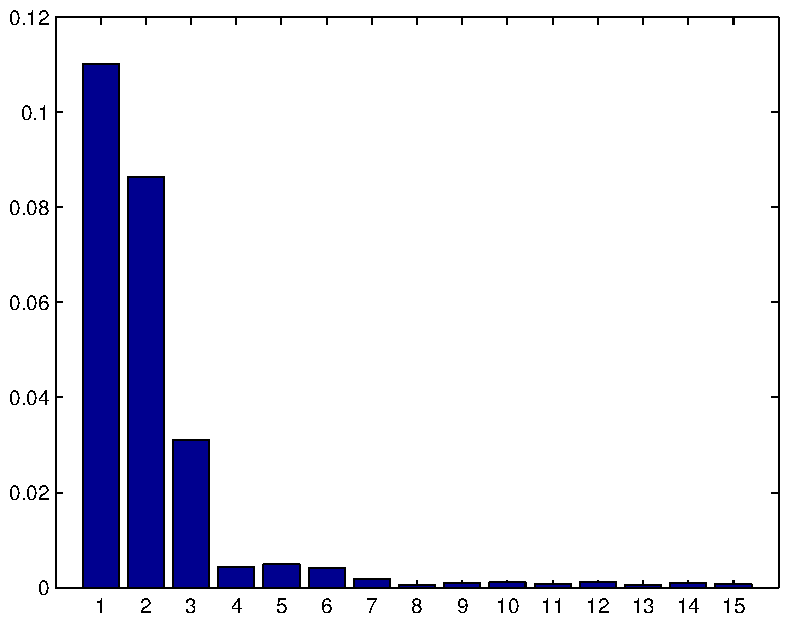
\includegraphics[width=0.145\textwidth]{../diagrams/Yale1Face/scales}
	\label{fig:yaleOneFaceScales}
}
\hspace{-5pt}
\subfigure[]{
	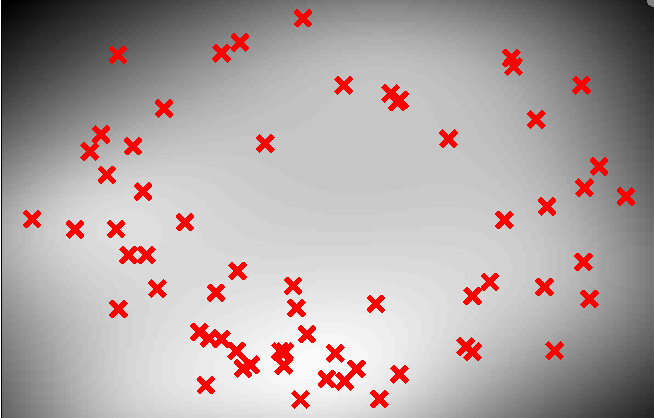
\includegraphics[width=0.145\textwidth]{../diagrams/Yale1Face/X21}
	\label{fig:yaleOneFaceX21}
}
\hspace{-5pt}
\subfigure[]{
	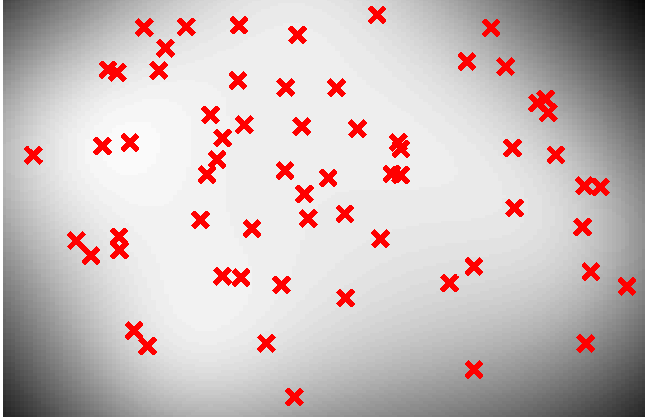
\includegraphics[width=0.145\textwidth]{../diagrams/Yale1Face/X23}
	\label{fig:yaleOneFaceX23}
}
\end{center}
\vspace{-7pt}
\caption{\small{ \it
The weight set $\bfw$ associated with the learned latent space is shown in \subref{fig:yaleOneFaceScales}.
In figures \subref{fig:yaleOneFaceX21} and \subref{fig:yaleOneFaceX23} we plotted pairs of the $3$ most dominant
latent dimensions against each other (dimension 1 against 2 and 1 against 3 respectively).
}
}
\label{fig:yaleOneFace1}
\vspace{-8pt}
\end{figure}
\hspace{-6pt}

This suggests that latent feature indices $1,2$ and $3$ encode the information about the illumination condition.
Figure \ref{fig:yaleOneFaceScales} also shows that the latent dimensions with indices $4,5$ and $6$ have a very small but not negligible weight.
%These are retained by the model because
%apart from the illumination condition, there exist other minor differences among pictures of a single face, as the depicted %persons
These represent other minor differences between an individual's face pictures, as the subjects
often blink, slightly move or smile etc. 



\subsubsection{Shared latent spaces for multiple faces}

In this section we use our model, from now on referred to as \emph{Manifold Relevance Determination model (MRD)} for latent subspace learning. 
We selected the pictures corresponding to all illumination conditions of $3$ subjects and created a dataset $Y$, and similarly
for $Z$ (for $3$ different subjects).
In this way, we formed two datasets, $Y$ and $Z$, each consisting of all $64 \times 3$ images corresponding to
a set of three different faces, therefore, $Y, Z \in \mathbb{R}^{N \times D}$, $N = 192$, $D = 32,256$.
 We then aligned the datasets, so that each image from the
first dataset was randomly set to correspond to one of the three faces of the second dataset which are depicted in the same illumination condition. In that way, the model is not
explicitly forced to learn the correspondence between face characteristics.

\par The MRD model was initialised by concatenating the two datasets and then performing PPCA in $Q=14$ dimensions. After training, 
the dimensions of the learned latent space are weighted by the parameters of the generative mappings $f_Y$ and $f_Z$ as shown in figure \ref{fig:yale6SetsScales}.

\begin{figure}[ht]
\begin{center}
\subfigure[]{
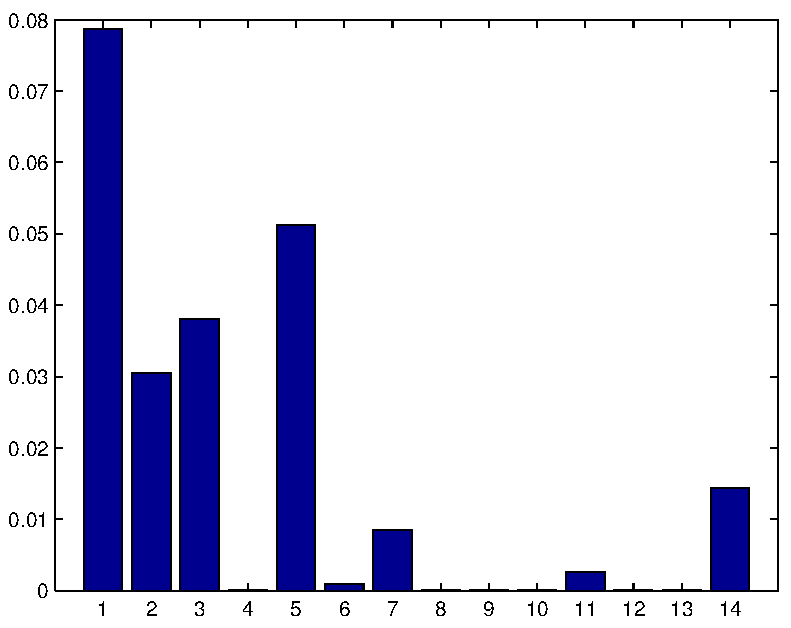
\includegraphics[width=0.18\textwidth]{../diagrams/Yale6Sets/scalesMod1}
	\label{fig:yale6SetsScales1}
}
\subfigure[]{
	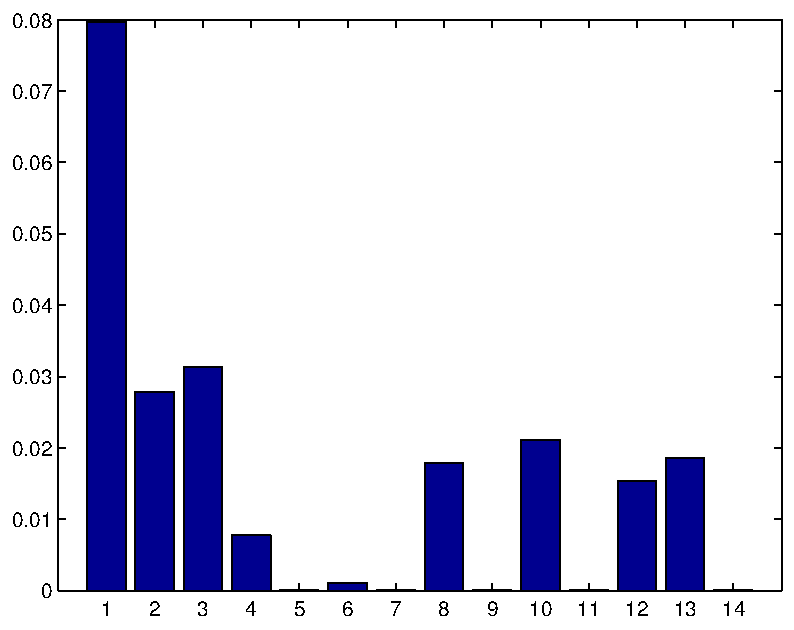
\includegraphics[width=0.18\textwidth]{../diagrams/Yale6Sets/scalesMod2}
	\label{fig:yale6SetsScales2}
}
\end{center}
\vspace{-9pt}
\caption{\small{ \it
The dimensions' weights, assigned for the first and second dataset 
in \subref{fig:yale6SetsScales1} and \subref{fig:yale6SetsScales2},
define a partitioning and ``soft'' sharing of the latent space. 
}}
\label{fig:yale6SetsScales}
\vspace{-8pt}
\end{figure}

The latent space is clearly segmented into a shared part, consisting of dimensions indexed as $1$,$2$ and $3$ 
\footnote{dimension 6 is also in the shared set but both models assigned a very small weight for that, as it encodes an almost negligible amount of information.}
and two private parts, consisting of dimensions indexed as $\{5,7,11,14 \}$ and $\{4,8,10,12,13 \}$ respectively. 
The $9$th feature of every latent point was found to be unnecessary for the generation of both output spaces.
What is more, 
the two models assigned almost (relatively) equal weights to the shared feature indices, and 
the shape of the shared latent space is similar to
the one found by the Bayesian GP-LVM (figure \ref{fig:yaleOneFace1}), as can be seen in figures \ref{fig:yale6SetsLatentSpace}\subref{fig:yale6SetsX12} and
\ref{fig:yale6SetsLatentSpace}\subref{fig:yale6SetsX13}.

This indicates that the shared space successfully encodes the information about
the position of the light source and not the face characteristics.
%as the random alignment that we performed forbade the algorithm from modelling commonalities between faces of the
%two different datasets.
 As for the private parts, these mainly correspond to disambiguating between faces of the same dataset. Indeed, plotting the largest two dimensions of
the first latent private subspace against each other reveals three clusters, corresponding to the three different faces within the dataset. 
Similarly to the standard Bayesian GP-LVM applied to a single face, here the private dimensions with the smaller weight
are the ones that model the minor differences introduced by the fact that the subject characteristics are slightly changed in several photos (due to blinking etc).

\hspace{-6pt}
\begin{figure}[ht]
\begin{center}
\subfigure[]{
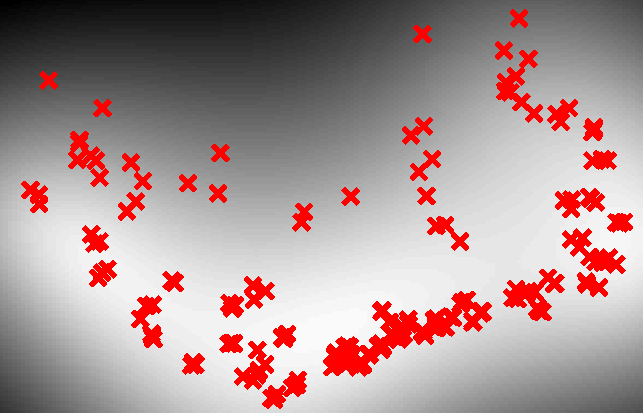
\includegraphics[width=0.145\textwidth]{../diagrams/Yale6Sets/mod1X_1_2}
	\label{fig:yale6SetsX12}
}
\hspace{-5pt}
\subfigure[]{
	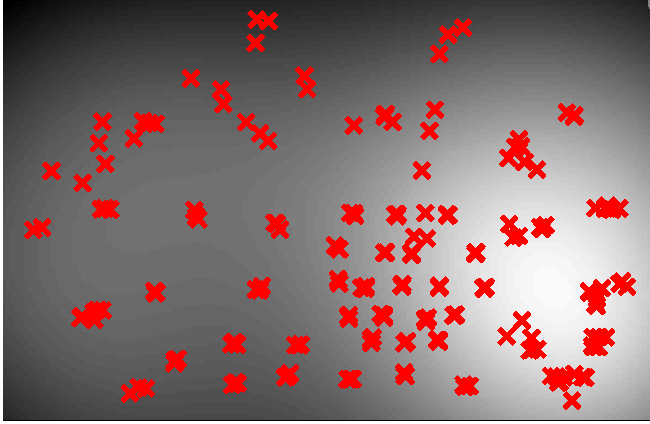
\includegraphics[width=0.145\textwidth]{../diagrams/Yale6Sets/mod1X_1_3}
	\label{fig:yale6SetsX13}
}
\hspace{-5pt}
\subfigure[]{
	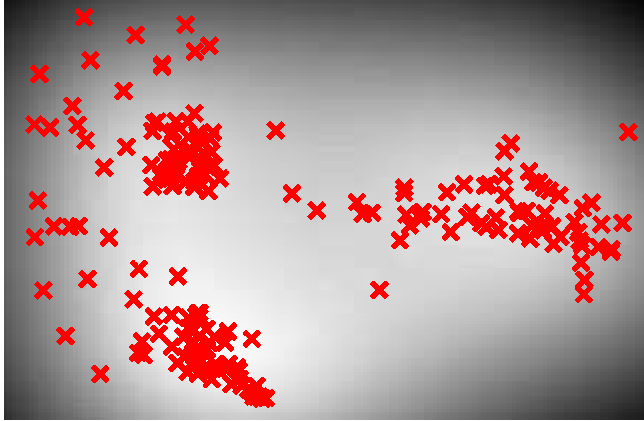
\includegraphics[width=0.145\textwidth]{../diagrams/Yale6Sets/mod1_X5_14}
	\label{fig:yale6SetsX5_14}
}
\end{center}
\vspace{-9pt}
\caption{\small{ \it
Projection of the shared latent space into dimensions $\{1,2\}$ and $\{1,3\}$ (figures
\subref{fig:yale6SetsX12} and \subref{fig:yale6SetsX13}) and projection of the $Y-$private dimensions $\{5,14\}$
(figure \subref{fig:yale6SetsX5_14}).
%which disambiguate between different faces in the first dataset.
 It is clear how the latent points in figure
\subref{fig:yale6SetsX5_14} form three clusters, each responsible for modelling one of the three faces in $Y$.
}}
\label{fig:yale6SetsLatentSpace}
\vspace{-8pt}
\end{figure}
\hspace{-6pt}


\par Given the above, it is obvious that the Manifold Relevance Determination model not only finds a very efficient and intuitive segmentation of the latent space, but it also
finds an effective dimensionality for each latent subspace. The Bayesian training allows for these procedures to be automated.

We can now confirm visually all of the subspaces' properties mentioned above and interpret their structure.
This is done by sampling a set of novel inputs $X_{samp}$ from each subspace and then mapping back to the observed data space using the
likelihood $p(Y|X_{samp})$, thus obtaining novel outputs (images).
%Being able to do so is an important advantage of our method (which is generative), because it also means that we can generate novel datapoints from the trained model.
%The intuitive segmentation of the latent space also helps towards this direction. 
To better understand what kind of information is encoded in each of the dimensions
of the shared or private spaces, we sampled new latent points by varying only one dimension at a time, while keeping the rest fixed. 

The first two rows of figure \ref{fig:yale6SetsInterpolation} show some of the outputs obtained after sampling across each of the shared dimensions $1$ and $3$ respectively, which clearly encode the coordinates of the light source,
whereas dimension $2$ was found to model the overall brightness. The sampling procedure can intuitively be thought as a walk in the space shown in figure \ref{fig:yale6SetsLatentSpace}\subref{fig:yale6SetsX13} from left to right and from the bottom to the top. Although the set of learned latent inputs is discrete, the corresponding latent subspace is continuous,
and we can interpolate images in new illumination conditions by sampling from areas where there are no training inputs (\ie in between the red crosses shown in figure \ref{fig:yale6SetsLatentSpace}).

% Using a generative model also allows us to sample new datapoints from the trained model. This is done by selecting a training input $\bfx_n$ (\ie one of
% the latent points corresponding to an existing, observed $\bfy_n$), and sampling one or more of its dimensions from the whole of the corresponding feature space,
% obtaining, thus, a novel input $\bfx_*$. We can then obtain novel outputs by using the likelihood $p(\bfy_n | \bfx_n)$. Figures \ref{}, \ref{} and \ref{} show some of the outputs obtained after
% sampling across each of the principle dimensions by hand. When the sampled $\bfx_*$ were close or exactly similar to training inputs, the corresponding output
% looks like one of the training datapoints, otherwise the output is novel. From the aforementioned figures, one can see that the two of the principal dimensions
% represent the change of the light source location along the $X$ and $Y$ axis respectively, whereas the third one is responsible for modelling the brightness.

Similarly, we can sample from the private subspaces and obtain novel outputs which interpolate the non-shared characteristics of the involved data. 
This results in a morphing effect across different faces, which is shown in the last row of figure \ref{fig:yale6SetsInterpolation}.
More examples and videos can be found in the supplementary material.


\begin{figure*}[ht]
\begin{center}
\subfigure{ 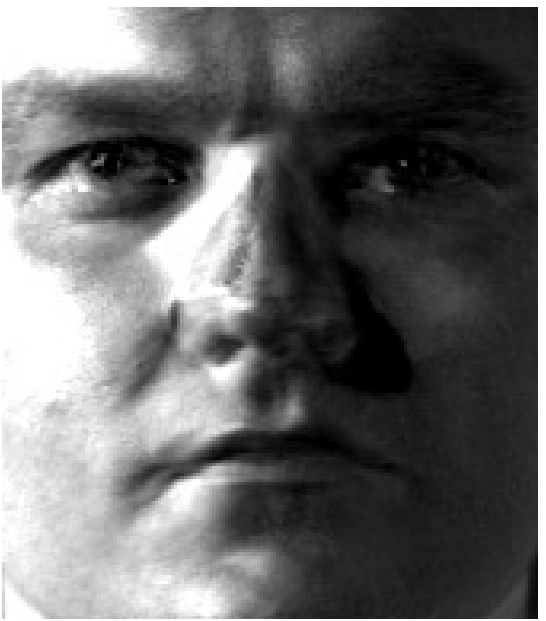
\includegraphics[width=0.09\textwidth]{../diagrams/Yale6Sets/lightInterpolation/X13_1000} }
\subfigure{ 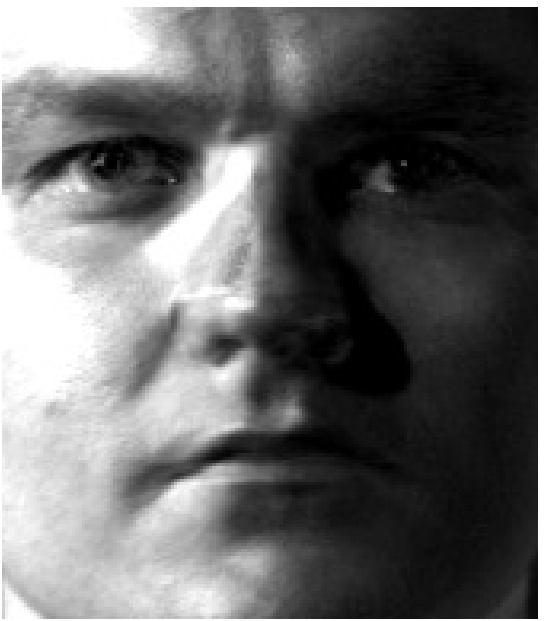
\includegraphics[width=0.09\textwidth]{../diagrams/Yale6Sets/lightInterpolation/X13_1009} }
\subfigure{ 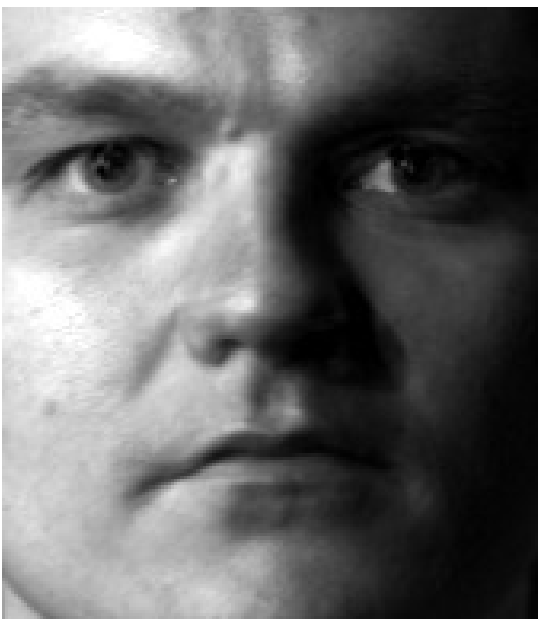
\includegraphics[width=0.09\textwidth]{../diagrams/Yale6Sets/lightInterpolation/X13_1021} }
\subfigure{ 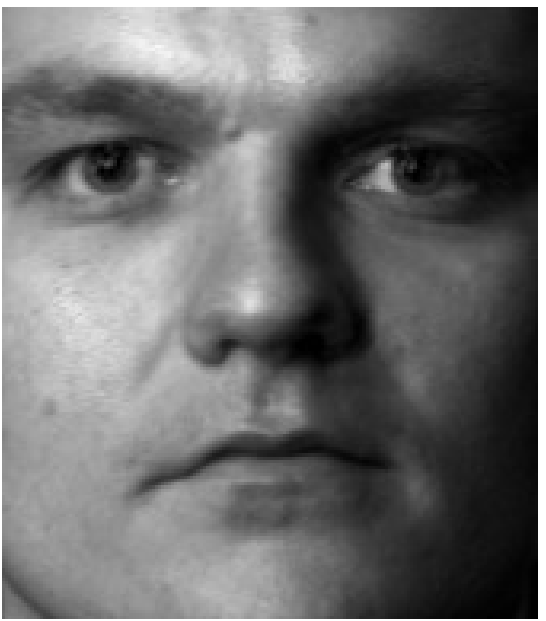
\includegraphics[width=0.09\textwidth]{../diagrams/Yale6Sets/lightInterpolation/X13_1022} }
\subfigure{ 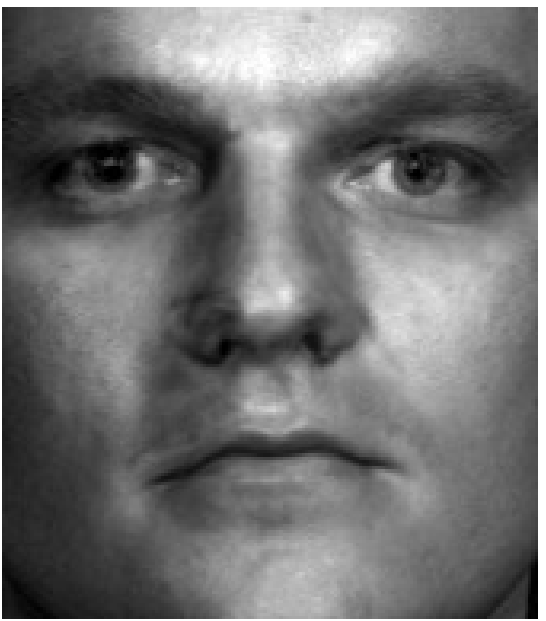
\includegraphics[width=0.09\textwidth]{../diagrams/Yale6Sets/lightInterpolation/X13_1036} }
\subfigure{ 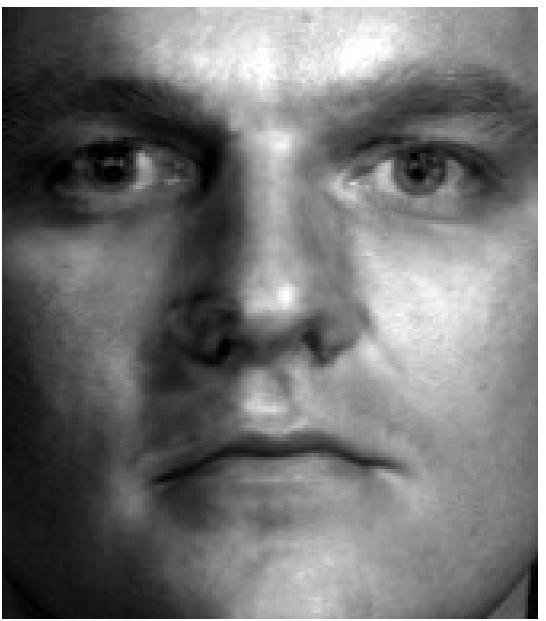
\includegraphics[width=0.09\textwidth]{../diagrams/Yale6Sets/lightInterpolation/X13_1040} }
\subfigure{ 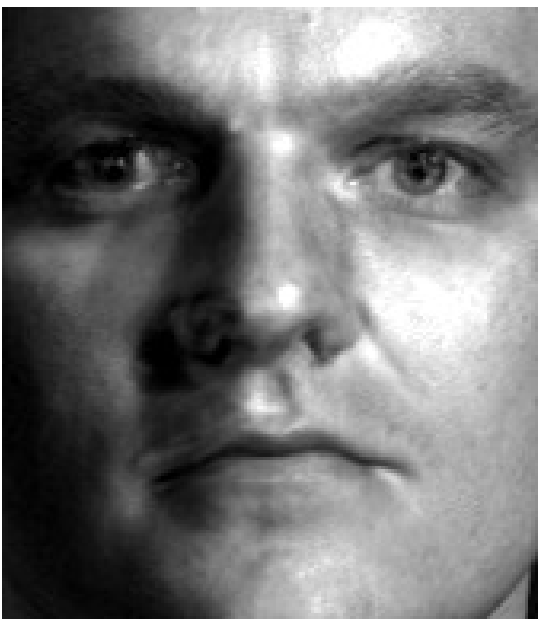
\includegraphics[width=0.09\textwidth]{../diagrams/Yale6Sets/lightInterpolation/X13_1046} }
\subfigure{ 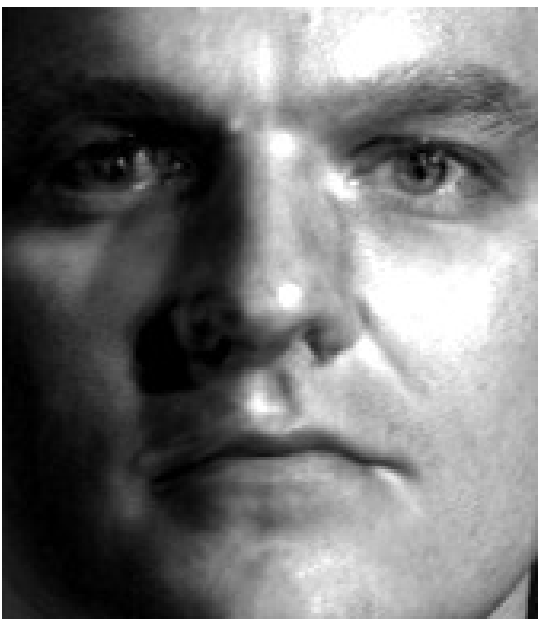
\includegraphics[width=0.09\textwidth]{../diagrams/Yale6Sets/lightInterpolation/X13_1055} }
\subfigure{ 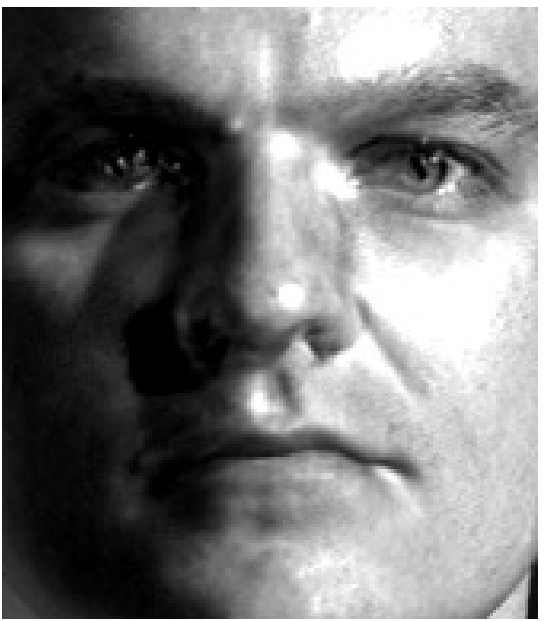
\includegraphics[width=0.09\textwidth]{../diagrams/Yale6Sets/lightInterpolation/X13_1063} }
\vspace{-8pt}
\newline
\subfigure{ 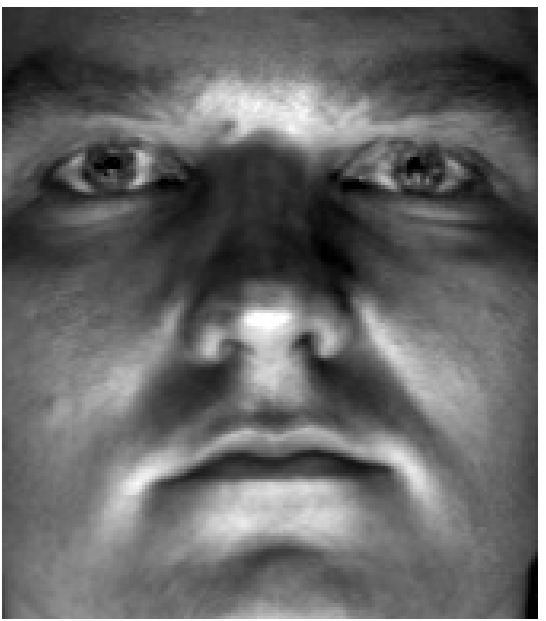
\includegraphics[width=0.09\textwidth]{../diagrams/Yale6Sets/lightInterpolation/X13_1064} }
\subfigure{ 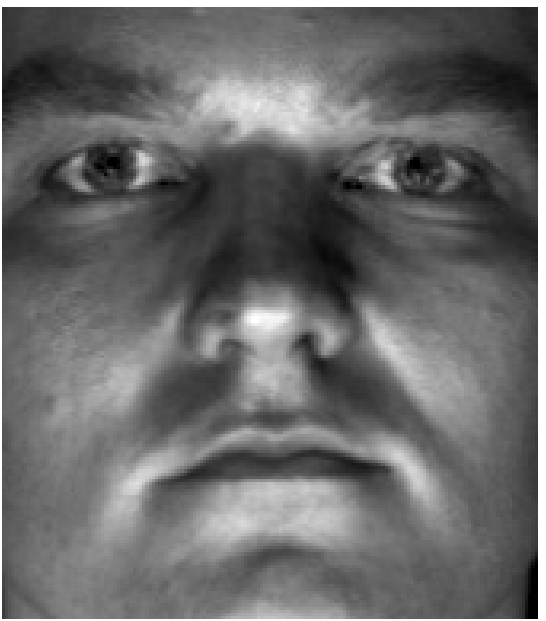
\includegraphics[width=0.09\textwidth]{../diagrams/Yale6Sets/lightInterpolation/X13_1072} }
\subfigure{ 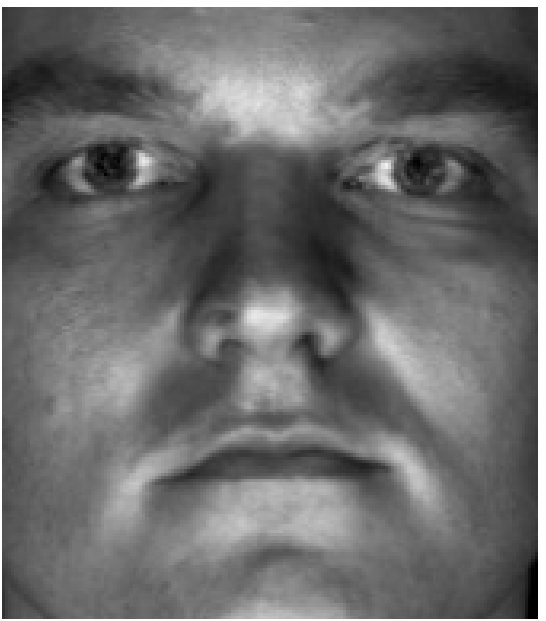
\includegraphics[width=0.09\textwidth]{../diagrams/Yale6Sets/lightInterpolation/X13_1079} }
\subfigure{ 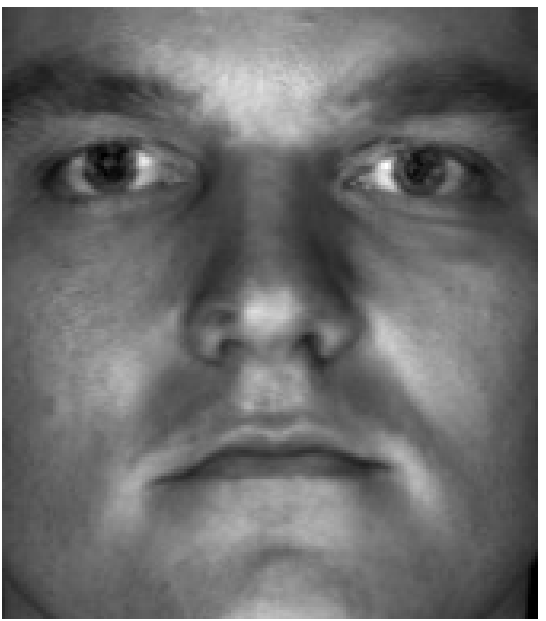
\includegraphics[width=0.09\textwidth]{../diagrams/Yale6Sets/lightInterpolation/X13_1085} }
\subfigure{ 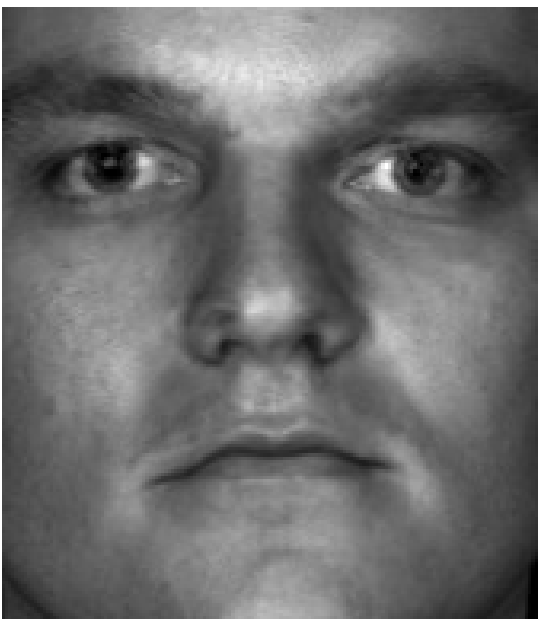
\includegraphics[width=0.09\textwidth]{../diagrams/Yale6Sets/lightInterpolation/X13_1095} }
\subfigure{ 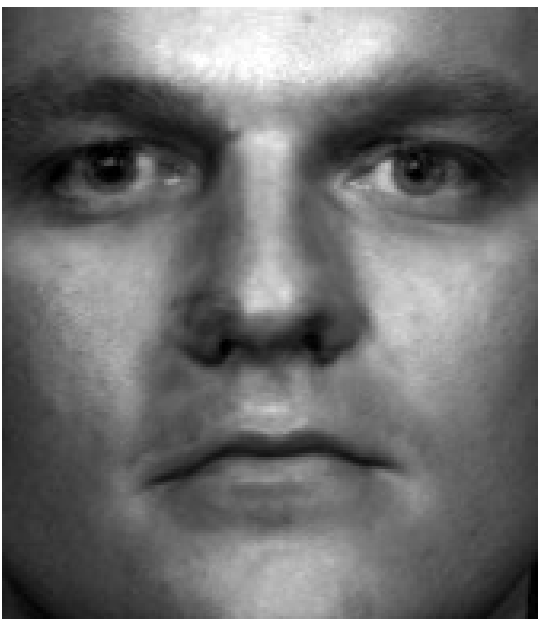
\includegraphics[width=0.09\textwidth]{../diagrams/Yale6Sets/lightInterpolation/X13_1110} }
\subfigure{ 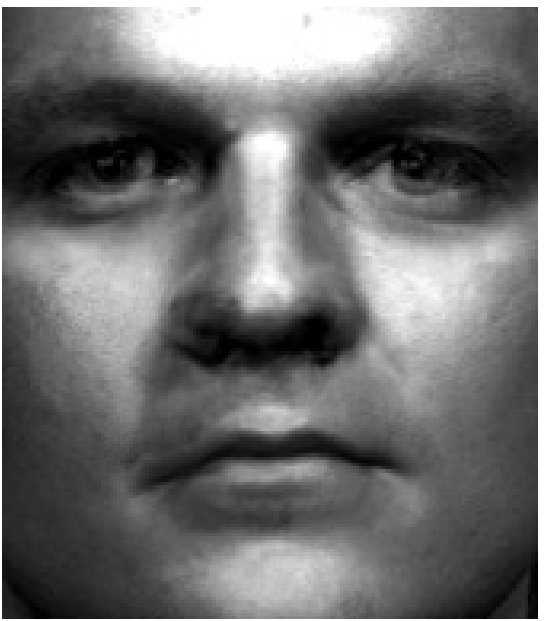
\includegraphics[width=0.09\textwidth]{../diagrams/Yale6Sets/lightInterpolation/X13_1125} }
\subfigure{ 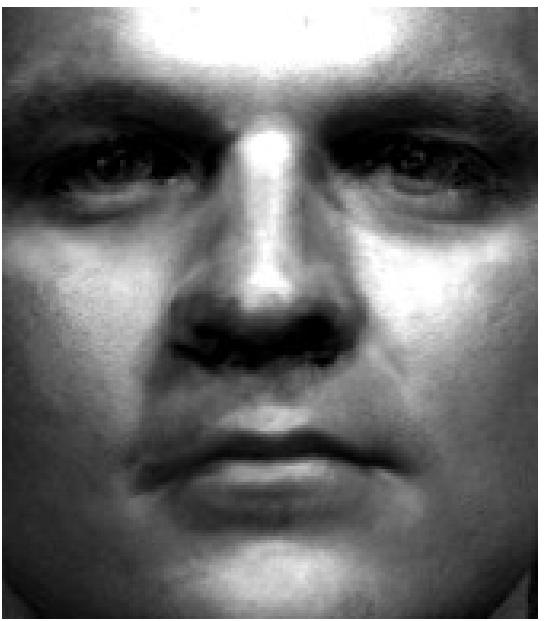
\includegraphics[width=0.09\textwidth]{../diagrams/Yale6Sets/lightInterpolation/X13_1137} }
\subfigure{ 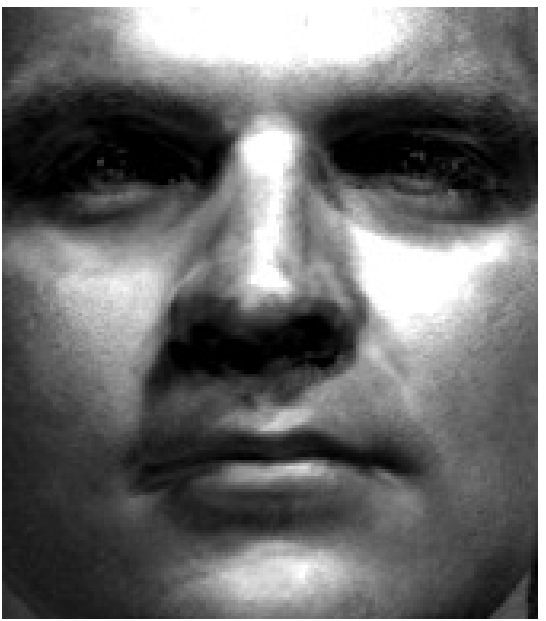
\includegraphics[width=0.09\textwidth]{../diagrams/Yale6Sets/lightInterpolation/X13_1149} }
\vspace{-8pt}
\newline
\subfigure{ 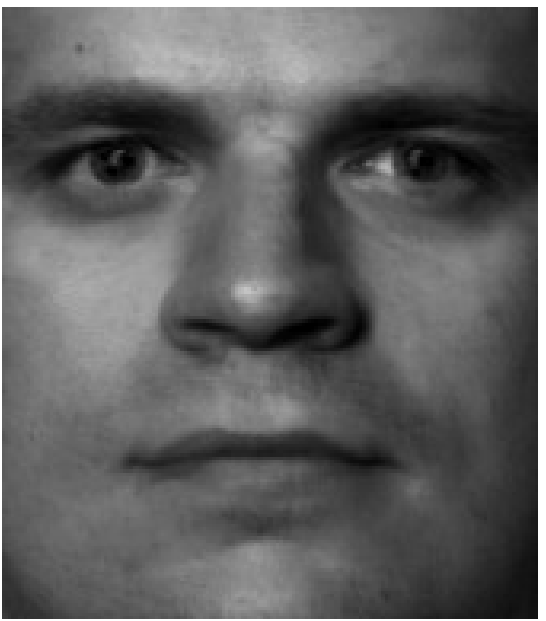
\includegraphics[width=0.11\textwidth]{../diagrams/Yale6Sets/morphing/1054} }
\subfigure{ 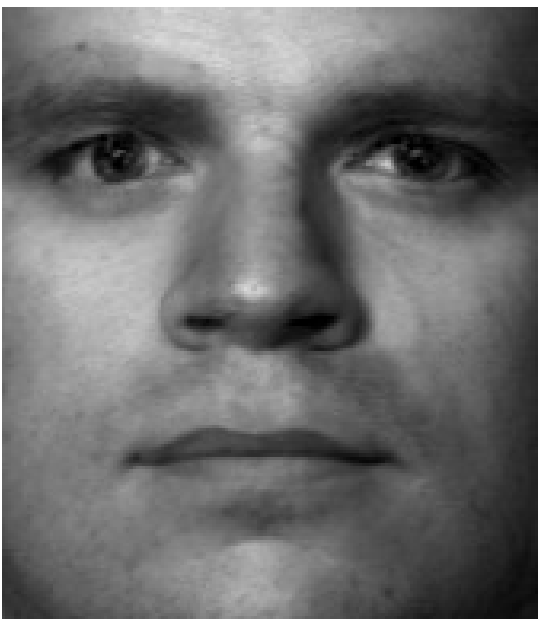
\includegraphics[width=0.11\textwidth]{../diagrams/Yale6Sets/morphing/1079} }
\subfigure{ 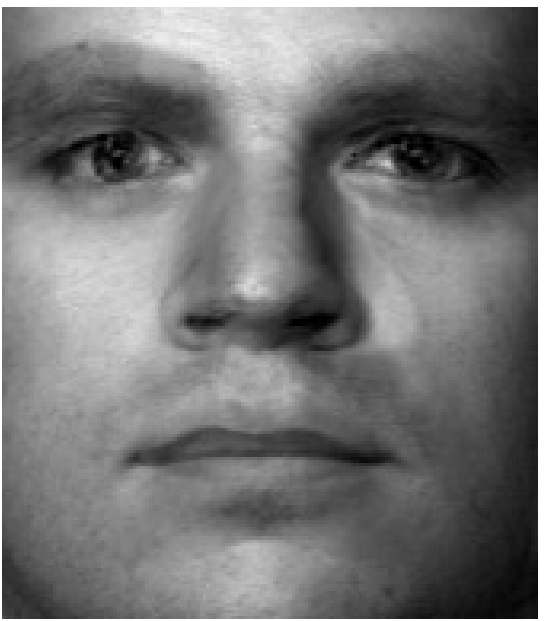
\includegraphics[width=0.11\textwidth]{../diagrams/Yale6Sets/morphing/1089} }
\subfigure{ 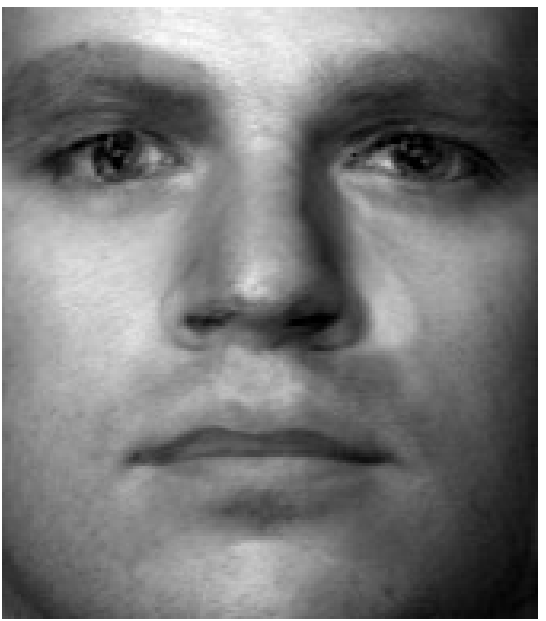
\includegraphics[width=0.11\textwidth]{../diagrams/Yale6Sets/morphing/1094} }
\subfigure{ 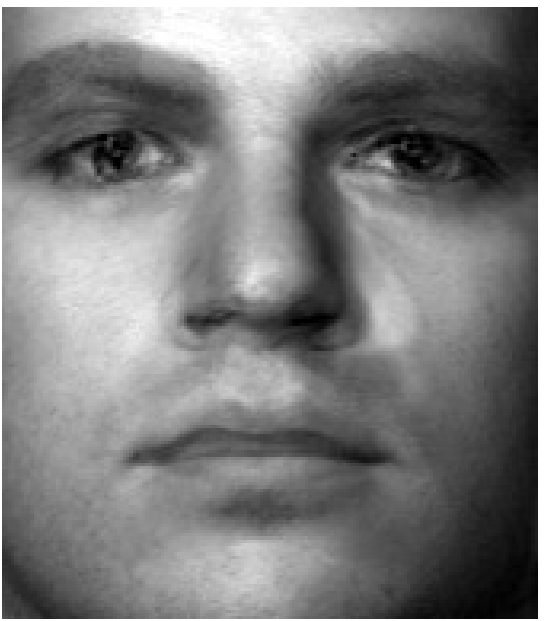
\includegraphics[width=0.11\textwidth]{../diagrams/Yale6Sets/morphing/1102} }
\subfigure{ 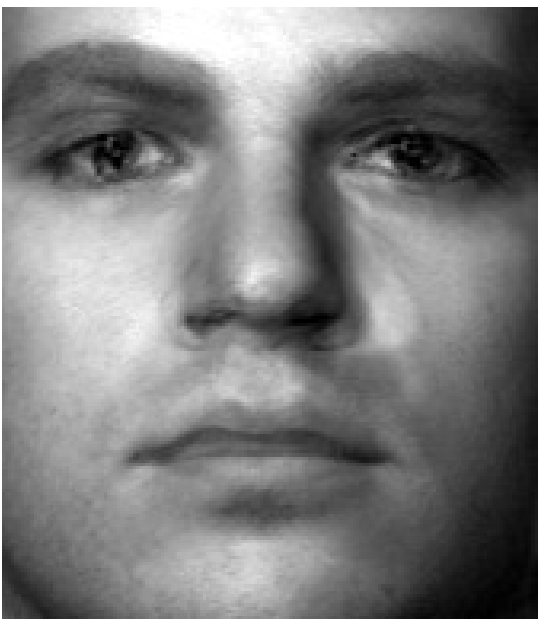
\includegraphics[width=0.11\textwidth]{../diagrams/Yale6Sets/morphing/1106} }
\subfigure{ 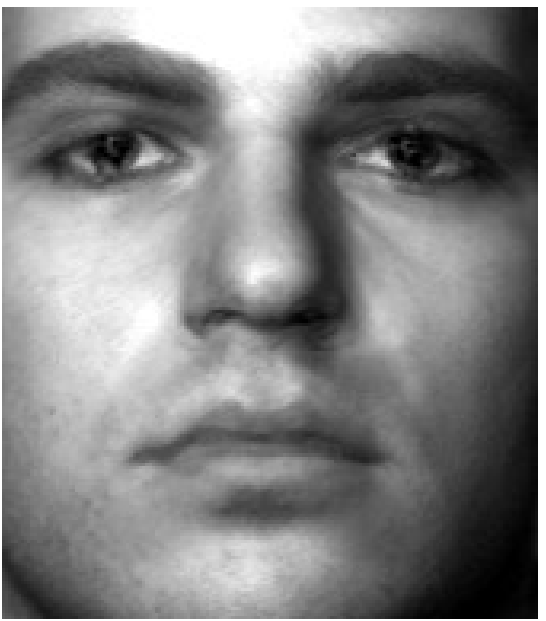
\includegraphics[width=0.11\textwidth]{../diagrams/Yale6Sets/morphing/1123} }
\end{center}
\vspace{-4pt}
\caption{\small{ \it
Sampling inputs to produce novel outputs.
First row shows interpolation between positions of the light source in the $x$ coordinate
and second row in the $y$ coordinate (elevation). Last row shows interpolation between
face characteristics to produce a morphing effect.
}}
\label{fig:yale6SetsInterpolation}
\vspace{-8pt}
\end{figure*}




\par As a final test, we confirm the efficient segmentation of the latent space into private and shared parts by automatically recovering all the illumination similarities found in
the training set.
 More specifically, given a datapoint $\bfy_n$ from the first dataset, we search the whole space of training inputs $X$ to find the $6$ Nearest Neigbours to the latent representation 
$\bfx_n$ of $\bfy_n$, based only on the shared dimensions. 
%In other words, we compare $x_{n,i}$ to all the rest $\{x_{n,j}\}_{n=1}^N$, where $i \neq j$ and $i,j$ belong to the set
% of the shared dimensions. 
 From these latent points, we can then obtain points in the output space of the second dataset, by using the likelihood $p(Z | X)$.
 As can be seen in figure \ref{fig:yale6SetsGrouping}, the model returns images which match
the illumination condition of the given image. Moreover, the fact that, typically, the first
neighbours of each given point correspond to outputs belonging to different faces, also indicates that
the shared latent space is ``pure'', and it does not encode similarities of face characteristics.
%\hspace{-6pt}
\begin{figure}[ht]
\begin{center}
\subfigure{ 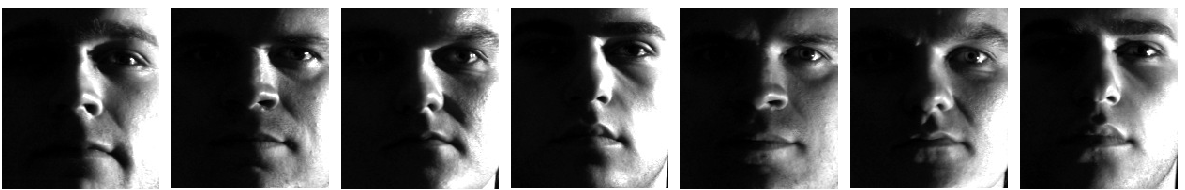
\includegraphics[width=0.47\textwidth]{../diagrams/Yale6Sets/grouping/givenMod2/122} }
 \vspace{-16pt}
 \newline
\subfigure{ 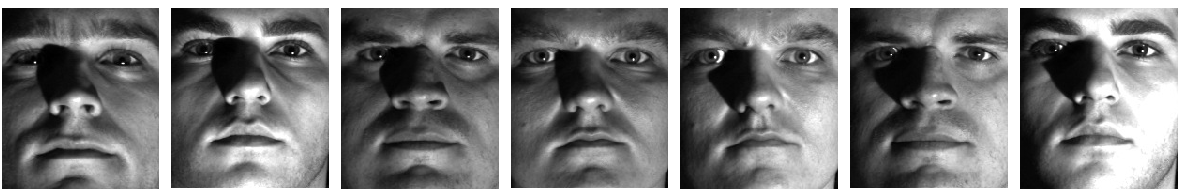
\includegraphics[width=0.47\textwidth]{../diagrams/Yale6Sets/grouping/givenMod2/107} }
 \vspace{-16pt}
 \newline
\subfigure{ 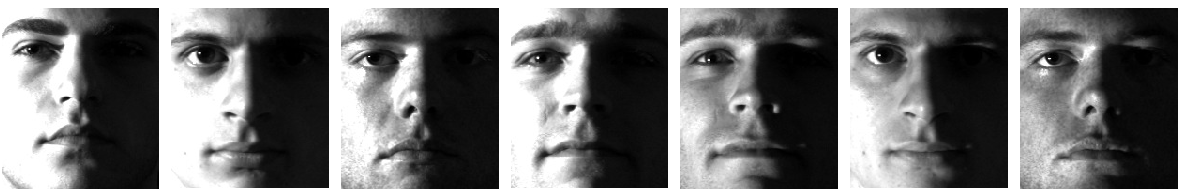
\includegraphics[width=0.47\textwidth]{../diagrams/Yale6Sets/grouping/givenMod1/24} }
 \vspace{-16pt}
 \newline
\subfigure{ 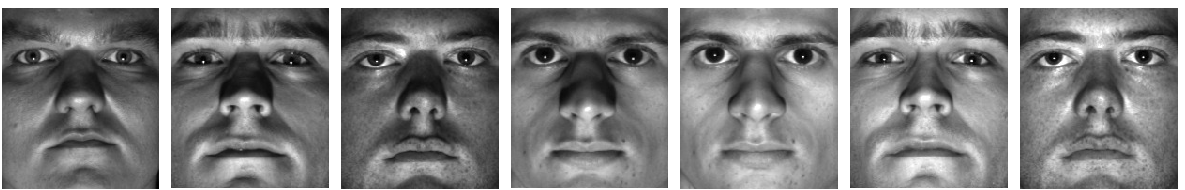
\includegraphics[width=0.47\textwidth]{../diagrams/Yale6Sets/grouping/givenMod1/70} }
 \vspace{-16pt}
 \newline
\end{center}
\vspace{-9pt}
\caption{\small{ \it
Given the images of the first column, the model searches only in the shared latent space to find the pictures of the opposite dataset
which have the same illumination condition. The images found, are sorted in columns
$2$ - $7$ by relevance.
}}
\label{fig:yale6SetsGrouping}
\vspace{-8pt}
\end{figure}

%\hspace{-6pt}

%%%% THE FIRST NN is the same latentn point, we should look from NN2 and so on.


\subsection{Human motion data}

For our second experiment, we consider 
a set of $3$D human poses and associated silhouettes,
coming from the dataset of Agarwal and Triggs \cite{Agarwal:pose06}. We used a subset of
$5$ sequences, totalling $649$ frames, corresponding to walking motions in various directions and patterns.
A separate walking sequence of $158$ frames was used as a test set.
Each pose is represented by a $63-$dimensional vector
of joint locations and each
silhouette is represented by a $100-$dimensional vector of HoG features.

\par Given the test silhouette features, we used our model to generate the corresponding
poses. This is a challenging task, since the data are multi-modal, \ie a silhouette representation
may be generated from more than one poses (\eg figure \ref{fig:humanPoseAmbiguity}). 

\begin{figure}[ht]
\begin{center}
%  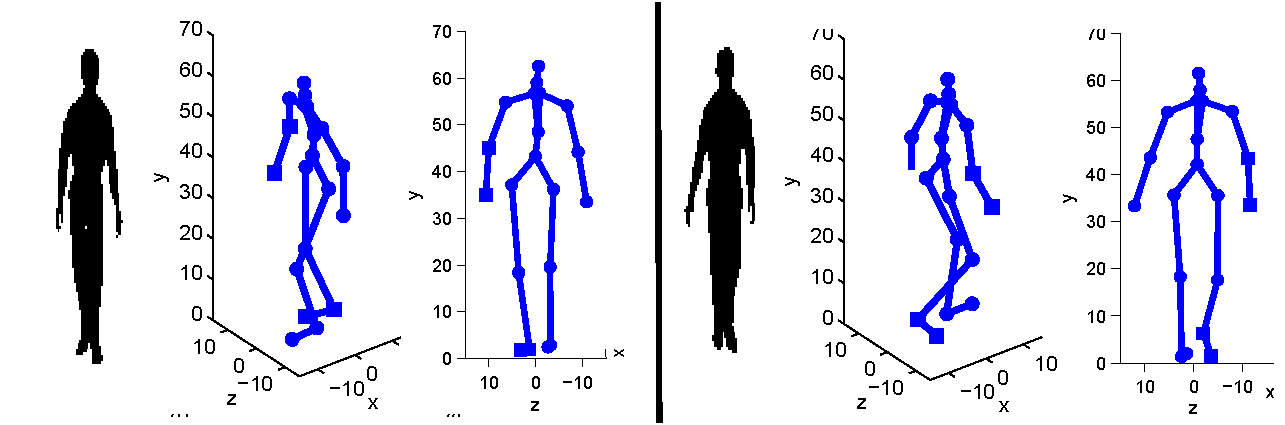
\includegraphics[width=0.43\textwidth]{../diagrams/humanPose/ambiguity2FinalCombined3}
  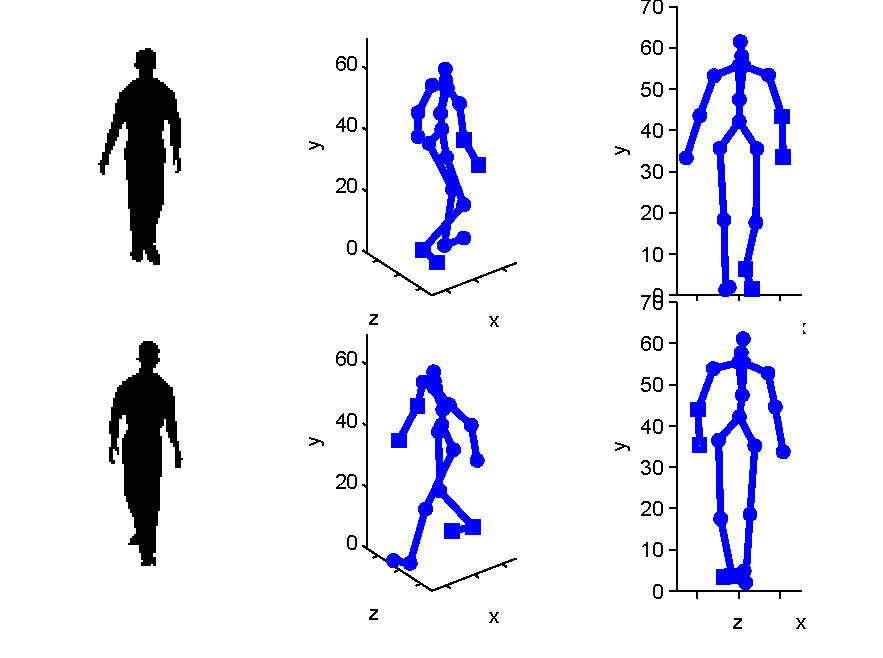
\includegraphics[width=0.35\textwidth]{../diagrams/humanPose/newAmbiguity}
\end{center}
\vspace{-9pt}
\caption{\small{ \it
Although the two poses in the second column are very dissimilar, they correspond to resembling silhouettes
that have similar feature vectors. This happens because the $3$D information is lost in the silhouette space,
as can also be seen in the third column, depicting the same poses from the silhouettes' viewpoint.}}
\label{fig:humanPoseAmbiguity}
\vspace{-4pt}
\end{figure}

As described in section \ref{inference}, given $\bfy^*$, one of the $N_*$ test silhouettes, our model optimises a test latent point $\bfx^*$ and finds
 a series of $K$ candidate initial training inputs $ \{ \bfx_{NN}^{(k)} \}_{k=1}^K$, sorted according to their similarity to $\bfx^*$, taking into account only the shared dimensions. 
 Based on these initial latent points, it then generates a sorted series of $K$ poses $\{ \bfzi^{(k)} \}_{k=1}^K$. For the dynamical version of our model,
all the test points are considered together and the predicted $N_*$ outputs are forced to form a smooth sequence.
 Our experiments showed that the initial training inputs $\bfx_{NN}$ typically correspond to silhouettes similar to the given one, something which
 confirms that the segmentation of the latent space is efficient. However, when ambiguities arise, as the example
 shown in figure \ref{fig:humanPoseAmbiguity}, the non-dynamical version of our model has no way of selecting the right one, since all points
 of the test sequence are treated independently. But when the dynamical version is employed, the model forces the whole set of training and test inputs to create smooth paths in the latent space, as can be seen in figure \ref{fig:humanPoseLatentSpaces}. In other words,
 the dynamics disambiguate the model.  

\begin{figure}[ht]
\begin{center}
\subfigure[]{ 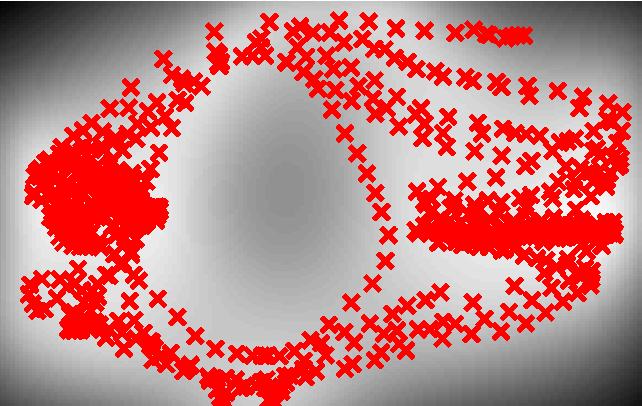
\includegraphics[width=0.18\textwidth]{../diagrams/humanPose/latentSpaceStatic} 
\label{fig:latentSpaceStatic}
} \hspace{-3pt}
\subfigure[]{ 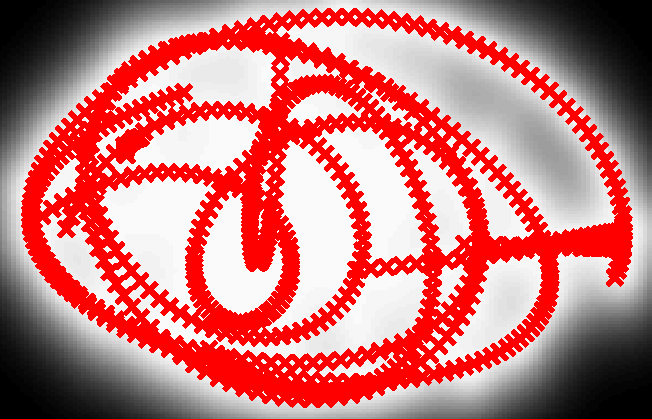
\includegraphics[width=0.18\textwidth]{../diagrams/humanPose/latentSpaceDynCropped} 
\label{fig:latentSpaceDyn}
}
\end{center}
\vspace{-9pt}
\caption{\small{ \it Projection of the latent space discovered for the non-dynamical model \subref{fig:latentSpaceStatic}
and for the dynamical model \subref{fig:latentSpaceDyn} onto their two principal dimensions.
}
}
\label{fig:humanPoseLatentSpaces}
\vspace{-3pt}
\end{figure}


Indeed, as can be seen in figure \ref{fig:humanPoseAmbiguityTest}, our method is forced to select a candidate training input $\bfx_{NN}$ for initialisation which does not necessarily
correspond to the training silhouette that is most similar to the test one. 
%
%In other words, the predicted pose is generated by a latent point which is not
%necessarily initialised in the latent point that is found by Nearest Neighbour in the silhouette space. 
%
What is more, if we assume that the test \emph{pose} $\bfzi^*$ is known and seek for its nearest training neighbour in the pose space, we find that the corresponding silhouette
is very similar to the one found by our model, which is only given information in the silhouette space.

\begin{figure}[ht]
\begin{center}
  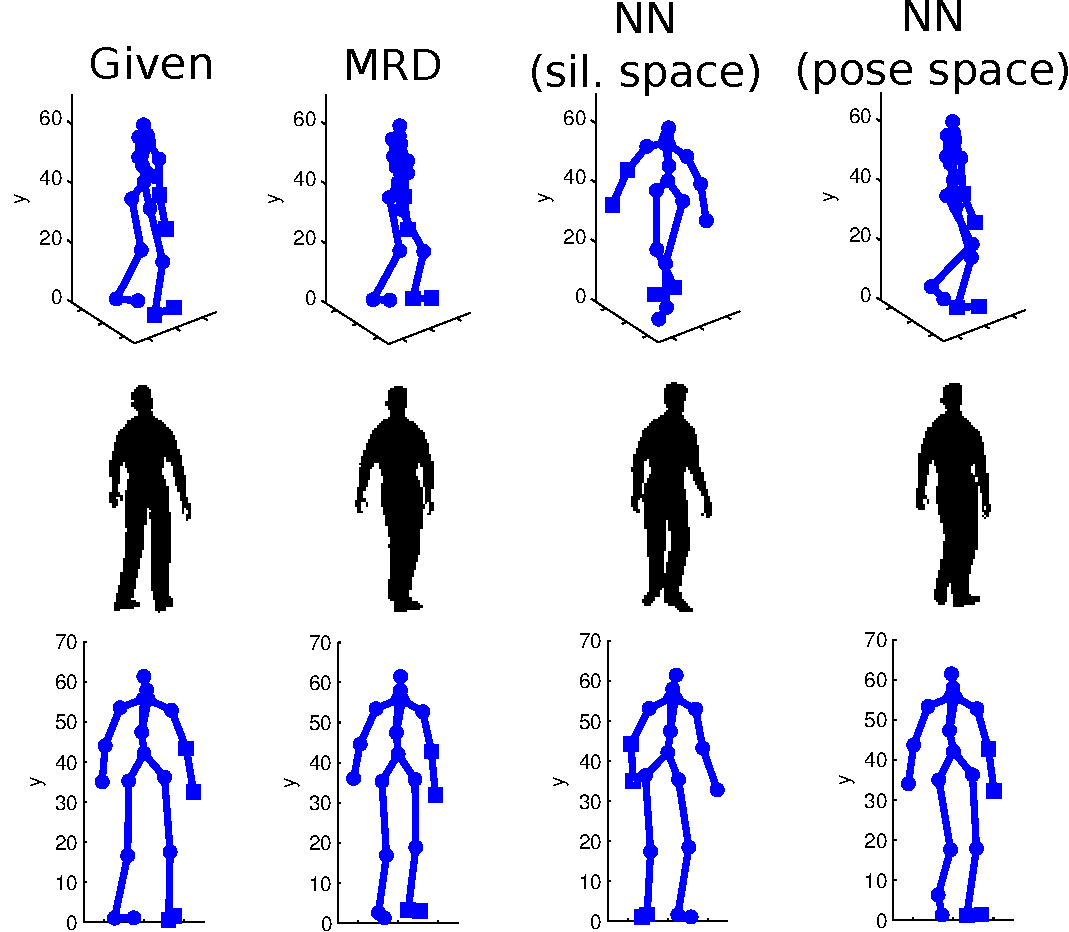
\includegraphics[width=0.35\textwidth]{../diagrams/humanPose/ambiguityTest}
\end{center}
\caption{\small{\it Given the HoG features for the test silhouette in column one, we predict the corresponding pose using the dynamical version of MRD and Nearest Neighbour in the silhouette space
obtaining the results in the first row, columns 2 and 3 respectively. The last row is the same as the first one, but the poses are rotated
to highlight the ambiguities. Notice that the silhouette shown in the second row for MRD does not correspond exactly to the pose
of the first row, as the model generates only the pose given a test silhouette. Instead, it is the training silhouette which MRD chose to initialise with, by performing
Nearest Neighbour in the shared latent space. 
We also found the Nearest Neighbour of the training \emph{pose} (column 4) given the test pose, so as to show that the corresponding silhouette is very similar to the one
selected by MRD for initialisation.
}}
\label{fig:humanPoseAmbiguityTest}
\end{figure}

\par Given the above, we quantify the results and compare our method
with linear and Gaussian process regression and Nearest Neighbour in the silhouette space. We also compared against
the Shared GP-LVM \cite{Ek:2008up, Ek:2009vv} which optimises the latent points using MAP and, therefore, requires an initial factorisation
of the inputs to be given a priori. 
The errors shown in table \ref{humanMotionTable} as well as the video provided as supplementary  material show that MRD
performs better than the other methods in this task.



\begin{table}[h]
\label{humanMotionTable}
\begin{center}
\begin{tabular}{|l|l|}
\hline
						 	   & Error \\ \hline \hline
Mean Training Pose		       & 6.16   \\ \hline
Linear Regression		       & 5.86   \\ \hline
GP Regression 			       & 4.27   \\ \hline
Nearest Neighbour (sil. space) & 4.88  \\ \hline
\textcolor{Gray}{Nearest Neighbour (pose space)} & \textcolor{Gray}{2.08}   \\ \hline
Shared GP-LVM				       & 5.13    \\ \hline
MRD	without Dynamics       & 4.67   \\ \hline
MRD with Dynamics	       & \textbf{2.94}    \\ \hline
\end{tabular}
\end{center}
\caption{
\small{ \it
The mean of the Euclidean distances of the joint locations between the predicted and the true poses.
The Nearest Neighbour in the pose space
is not a fair comparison, but is reported here as it provides some insight about the
lower bound on the error that can be achieved for this task.
}}
\end{table}








